%%%%%%%%%%%%%%%%%%%%%%%%%%%%%%%%%%%%%%%%%%%%%%%%%%%%%%%%%%%%%%%%%%%%%%%%%%%%%%%%%%%%%%%%%%%%%%%%
%
% CSCI 1430 Written Question Template
%
% This is a LaTeX document. LaTeX is a markup language for producing documents.
% Your task is to answer the questions by filling out this document, then to 
% compile this into a PDF document. 
% You will then upload this PDF to `Gradescope' - the grading system that we will use. 
% Instructions for upload will follow soon.
%
% 
% TO COMPILE:
% > pdflatex thisfile.tex
%
% If you do not have LaTeX and need a LaTeX distribution:
% - Departmental machines have one installed.
% - Personal laptops (all common OS): http://www.latex-project.org/get/
%
% If you need help with LaTeX, come to office hours. Or, there is plenty of help online:
% https://en.wikibooks.org/wiki/LaTeX
%
% Good luck!
% James and the 1430 staff
%
%%%%%%%%%%%%%%%%%%%%%%%%%%%%%%%%%%%%%%%%%%%%%%%%%%%%%%%%%%%%%%%%%%%%%%%%%%%%%%%%%%%%%%%%%%%%%%%%
%
% How to include two graphics on the same line:
% 
% \includegraphics[width=0.49\linewidth]{yourgraphic1.png}
% \includegraphics[width=0.49\linewidth]{yourgraphic2.png}
%
% How to include equations:
%
% \begin{equation}
% y = mx+c
% \end{equation}
% 
%%%%%%%%%%%%%%%%%%%%%%%%%%%%%%%%%%%%%%%%%%%%%%%%%%%%%%%%%%%%%%%%%%%%%%%%%%%%%%%%%%%%%%%%%%%%%%%%

\documentclass[11pt]{article}

\usepackage[english]{babel}
\usepackage[utf8]{inputenc}
\usepackage[colorlinks = true,
            linkcolor = blue,
            urlcolor  = blue]{hyperref}
\usepackage[a4paper,margin=1.5in]{geometry}
\usepackage{stackengine,graphicx}
\usepackage{fancyhdr}
\setlength{\headheight}{15pt}
\usepackage{microtype}
\usepackage{times}
\usepackage{amsmath}
\usepackage[shortlabels]{enumitem}
\setlist[enumerate]{topsep=0pt}

% a great python code format: https://github.com/olivierverdier/python-latex-highlighting
\usepackage{pythonhighlight}

\frenchspacing
\setlength{\parindent}{0cm} % Default is 15pt.
\setlength{\parskip}{0.3cm plus1mm minus1mm}

\pagestyle{fancy}
\fancyhf{}
\lhead{Project 2 Questions}
\rhead{CSCI 1430}
\lfoot{\textcolor{red}{Only 
\ifcase\thepage
\or instructions
\or E1 results
\or E1 results
\or A1(a)
\or A1(b)
\or A1(c)
\or A2
\or A3
\or A4(a,b,c)
\or A4(d)
\or A4(e)
\or feedback
\else
EXTRA PAGE ADDED
\fi
should be on this page
}}
\rfoot{\thepage~/ 12}

\date{}

\title{\vspace{-1cm}Project 2 Questions}


\begin{document}
\maketitle
\vspace{-3cm}
\thispagestyle{fancy}

\section*{Instructions}
\begin{itemize}
  \item One exercise graded for completion only.
  \item Four graded questions.
  \item Write code where appropriate.
  \item Feel free to include images or equations.
  \item Please make this document anonymous.
  \item This assignment is \textbf{fixed length}, and the pages have been assigned for you in Gradescope. As a result, \textbf{please do NOT add any new pages}. We will provide ample room for you to answer the questions. If you \emph{really} wish for more space, please add a page \emph{at the end of the document}.
  \item \textbf{We do NOT expect you to fill up each page with your answer.} Some answers will only be a few sentences long, and that is okay.
\end{itemize}


\section*{Exercise}

\paragraph{E1:} Let's look again at the webcam Fourier decomposition demo which James showed in class. Let's run it in our CSCI 1430 virtual environment from within the 'questions' directory. \emph{Preferably, use a computer with a webcam}; if you don't have a webcam, the software will use a static image.

\begin{verbatim}
$ python liveFFT2.py
\end{verbatim}

This file contains five parts for you to explore and see the amplitude image, the phase image, and the effect of the reconstructed image.
\begin{itemize}
    \item Part 0: Scanning the basis and observing the output image.
    \item Part 1: Reconstructions from different numbers of basis frequencies.
    \item Part 2: Replacing amplitude and phase with that from a different image.
    \item Part 3: Replacing amplitude and phase with that from a noise image.
    \item Part 4: Manipulating the amplitude and phase images.
\end{itemize}

Uncomment the different parts and explore the camera feed decomposition! Please include the results of your experimentation, e.g., two-to-three screenshots of what you discover. We'll be grading for completion, not correctness. \emph{Note:} For anonymous grading, try not to put yourself in the camera frame. Show your favourite vector calculus book, wear a mask, use your cat, etc. Extra credit for creative effort.

%%%%%%%%%%%%%%%%%%%%%%%%%%%%%%%%%%%

% Please leave the pagebreak
\pagebreak
\section*{Exercise Results}
Please include images of your results from the exercise here, e.g., two-to-three screenshots of your findings.

The image is taken from the recent released album of IU, celebrity! (The best song ever this year!)

Part 0: in part 0, only one basis sine wavefunction is used in experimentation. We could see that the bottom-left and bottom-right are both black because the amplitude and phase are both zeros. The top-right shows black-white stripes that are resulted from the sine wavefunction that we selected.  

% 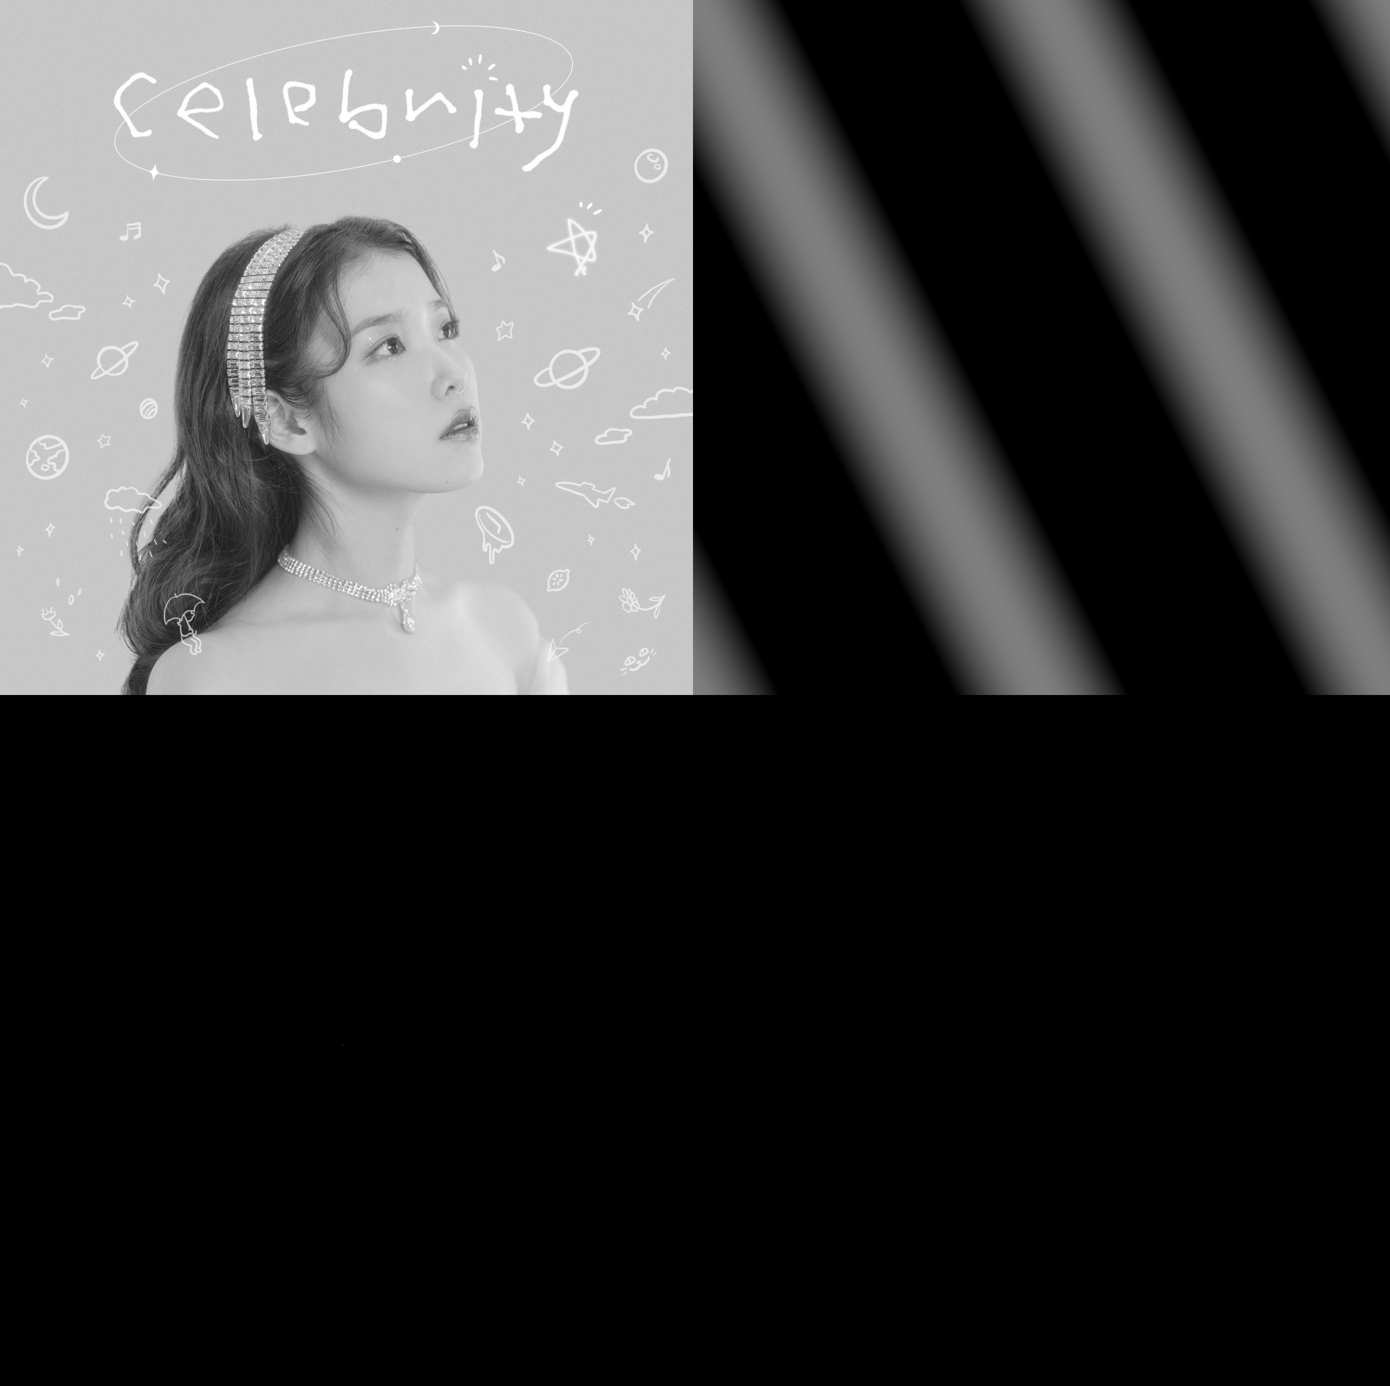
\includegraphics[width=0.49\linewidth]{Part0.png}

Part 1: in part 1, we construct the image using different numbers of basis frequencies. The radius of the circle in bottom-left can represent the number of basis frequencies that we used in reconstruction of the image. (the black part is because we set amplitudes of other frequencies as 0) As the figure shown below(left), when we only use a small portion of frequencies, the reconstructed image is blurred. On the contrary, when more frequencies is used, the image will become clearer.

\begin{figure*}[htbp]
    \centering
    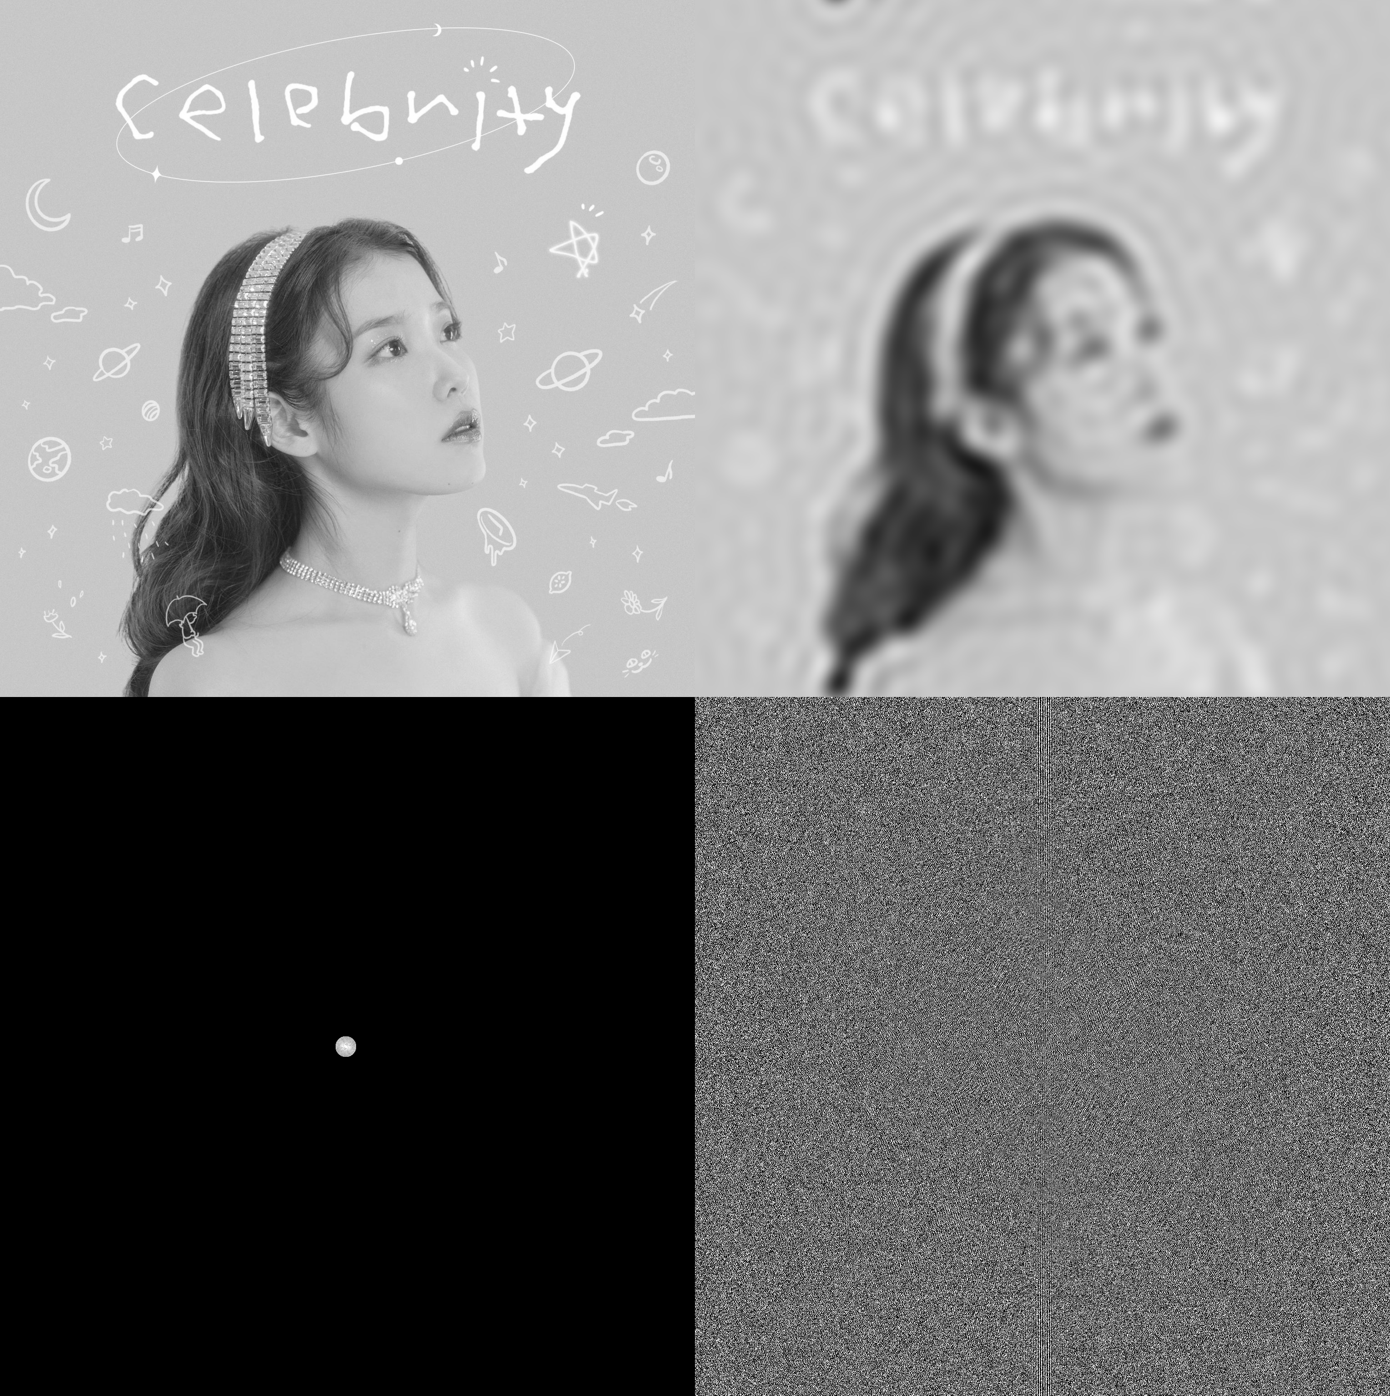
\includegraphics[width=0.49\linewidth]{Part1_small_radius.png}
    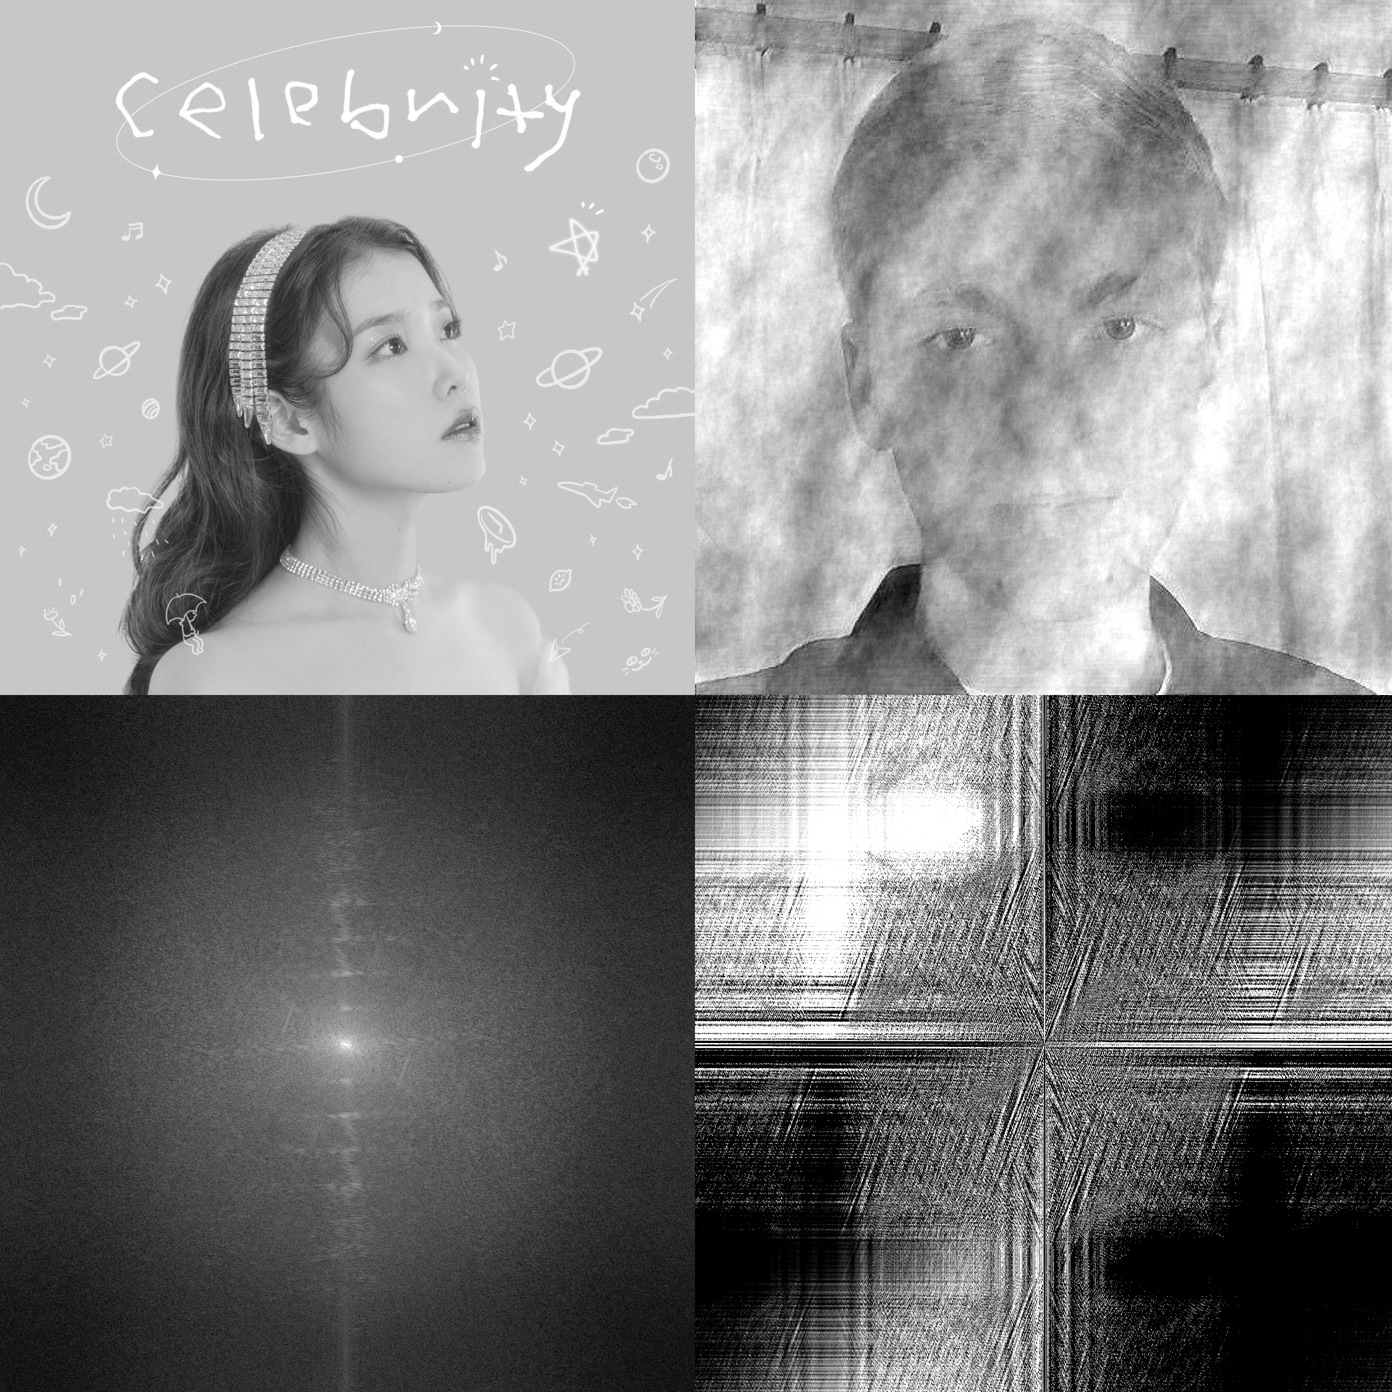
\includegraphics[width=0.49\linewidth]{Part2_phase.png}
    \caption{Left: result of part 1; Right: result of part 2 replacing phase with Jackimage}
\end{figure*}

% 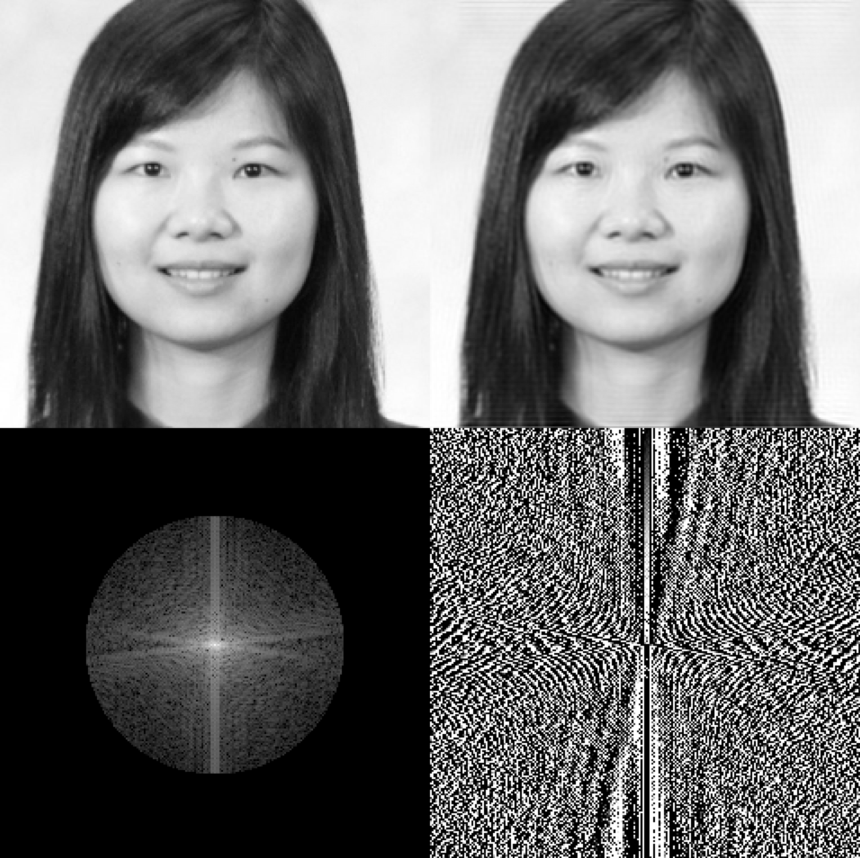
\includegraphics[width=0.49\linewidth]{Part1_large_radius.png}


Part 2: in part 2, we replace the amplitude and phase with other image ("JacksonGibbonsCrop.png" in this case). The results are very interesting. When we only replace the amplitude, the reconstructed image still show original content (IU's face in this case) but with some blurred shadow over the image. When we only replace the phase, the reconstructed image shows the content in the new image (Jack's face in this case, shown in Fig. 1 Right). And when we change both, the reconstructed image is totally the new image content, which is quite obviously as we have changed all the information in FFT step.
In this part, it may imply that the phase is more impoartant to reconstruct the image than the amplitude as when we replace phase we totally lost the original information.

\pagebreak
Part 3: in part 3, we replace the amplitude and phase with that of a noisy image. This is quite similar to what we have done in Part 2. When we replace the amplitude, we can only see the edges of the face in the reconstructed image. When we replace the phase, we see random noisy points in the reconstructed image. And when we replace both, the reconstructed image is totally a random noisy image.


Part 4: in part 4, we have done many manipulation to the amplitude and phase of the image. Add phase value will add some mask layers to the reconstructed image . Flip the phase values will flip the reconstructed image as well. Rotate the phase values will result in the reconstructed image darker than the original. Rotate the whole image will result in the following reconstructed image (Fig. 2). It flips the image and add a darker stripe to the image as well.

\begin{figure}[htbp]
    \centering
    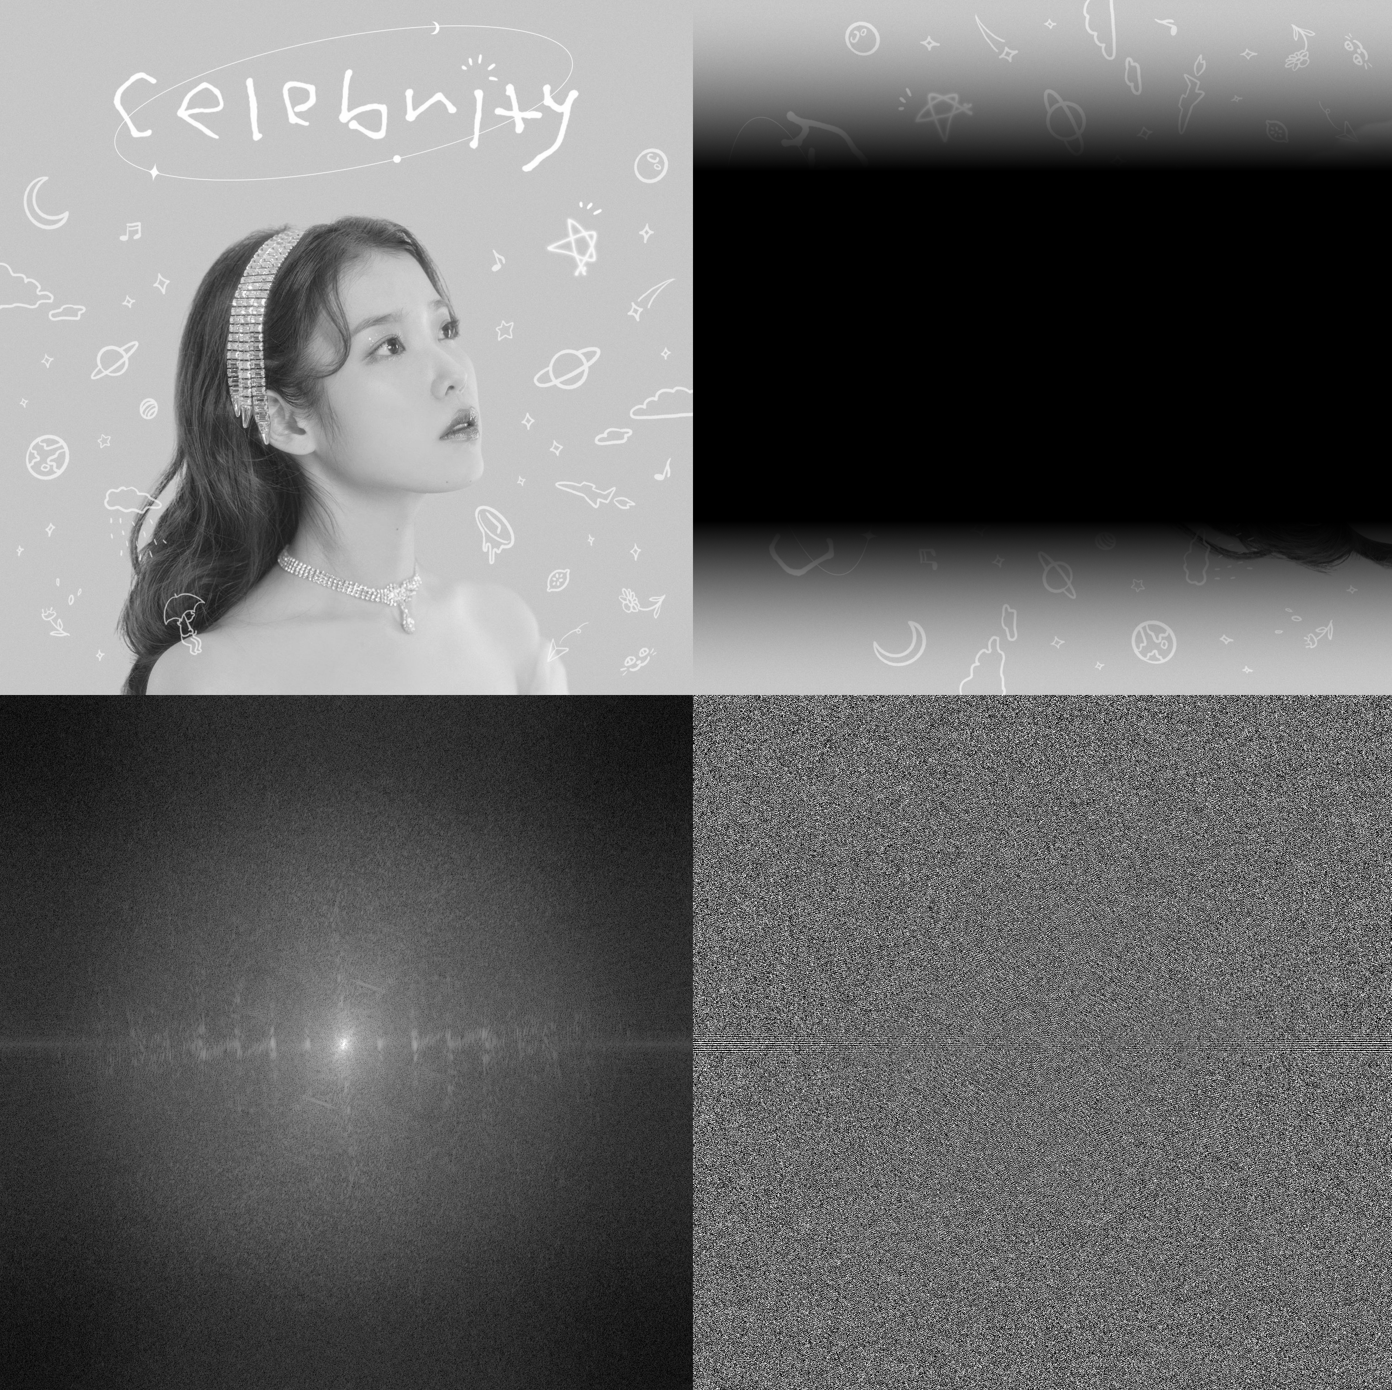
\includegraphics[width=0.5\linewidth]{Part4_rotate_whole_image.png}
    \caption{Rotate the phase values}
\end{figure}




%%%%%%%%%%%%%%%%%%%%%%%%%%%%%%%%%%%

% Please leave the pagebreak
\pagebreak
\section*{Questions}

\paragraph{Q1:} Imagine we wished to find points in one image which matched to the same world point in another image---so-called feature point correspondence matching. We are tasked with designing an image feature point algorithm which could match world points in the following three pairs of images.
\newline
\newline
\emph{RISHLibrary:} \href{RISHLibrary1.jpg}{One} \href{RISHLibrary2.jpg}{Two} | \emph{Chase:} \href{Chase1.jpg}{One} \href{Chase2.jpg}{Two} | \emph{LaddObservatory:} \href{LaddObservatory1.jpg}{One} \href{LaddObservatory2.jpg}{Two}

Please use the included python script \texttt{plot\_corners.py} to find corners using Harris corner detection for each image above.

For each pair, discuss the differences in the returned corners (if any), and what aspects of the images may have caused these differences. Then discuss what real world challenges exist in matching features between images.


%%%%%%%%%%%%%%%%%%%%%%%%%%%%%%%%%%%
\paragraph{A1 (a):} Answer for RISHLibrary pair

The results are shown in Fig. 3. The corners returned for \texttt{RISHLibrary1.jpg} and \texttt{RISHLibrary2.jpg} are different. In left part, the corners returned are corners on the person's shoes while in right part, the corners returned are the chairs' legs. This is because these two images show different content and we cannot find the same corners in these two images. And in both images, there are not enough corners to be detected because a large portion of the image is the flat floor. Challenges in real life: sometimes we will have to make sure the images we want to match actually showing the same content. Otherwise, matching would be meaningless. And it could be difficult to match images that don't have many corners as the algorithm might not be able to detect any corners to match.

\begin{figure*}[htbp]
    \centering
    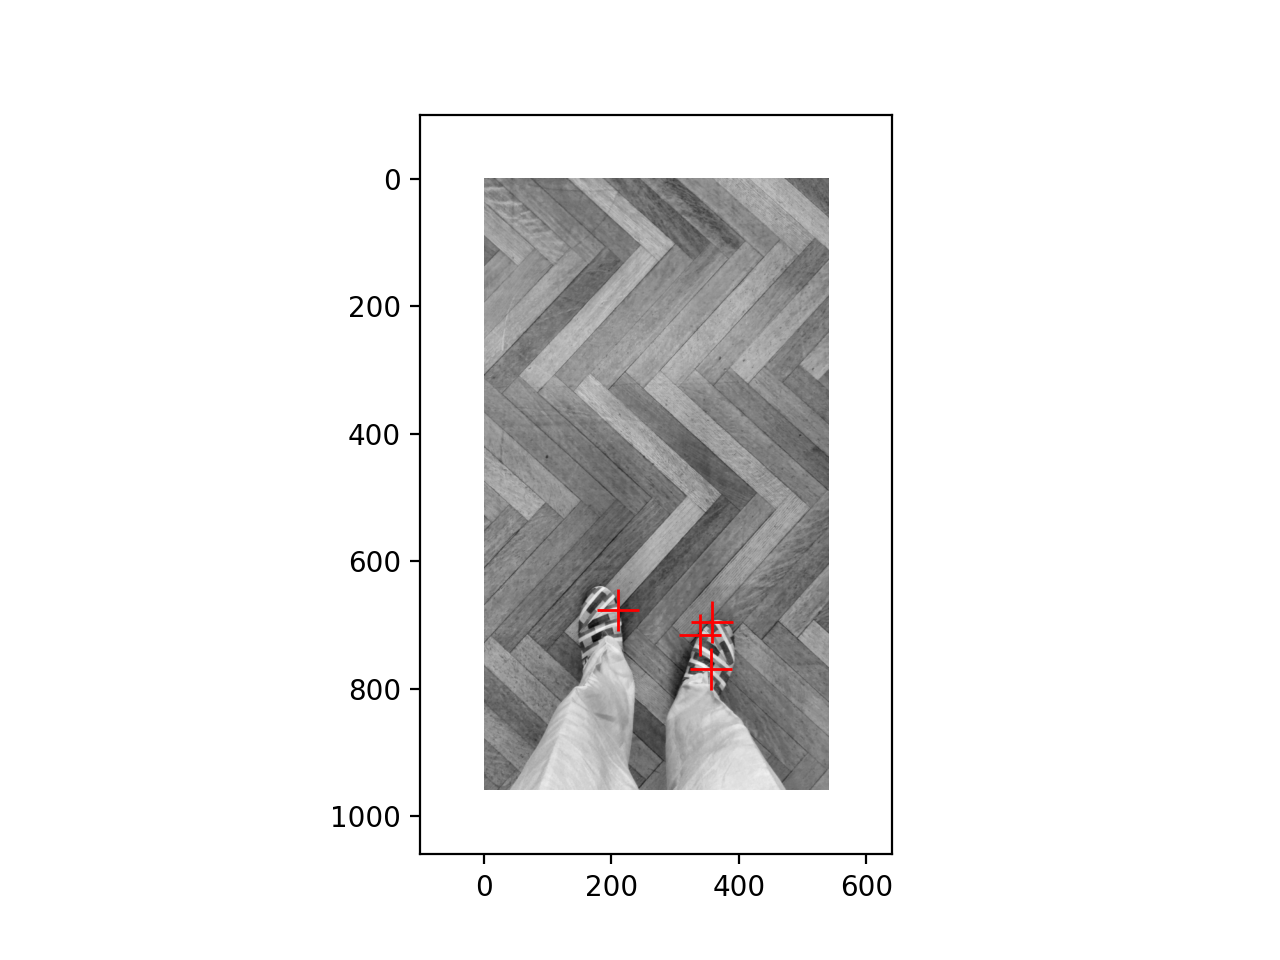
\includegraphics[width=0.49\linewidth]{Q1_RISHLibrary1.png}
    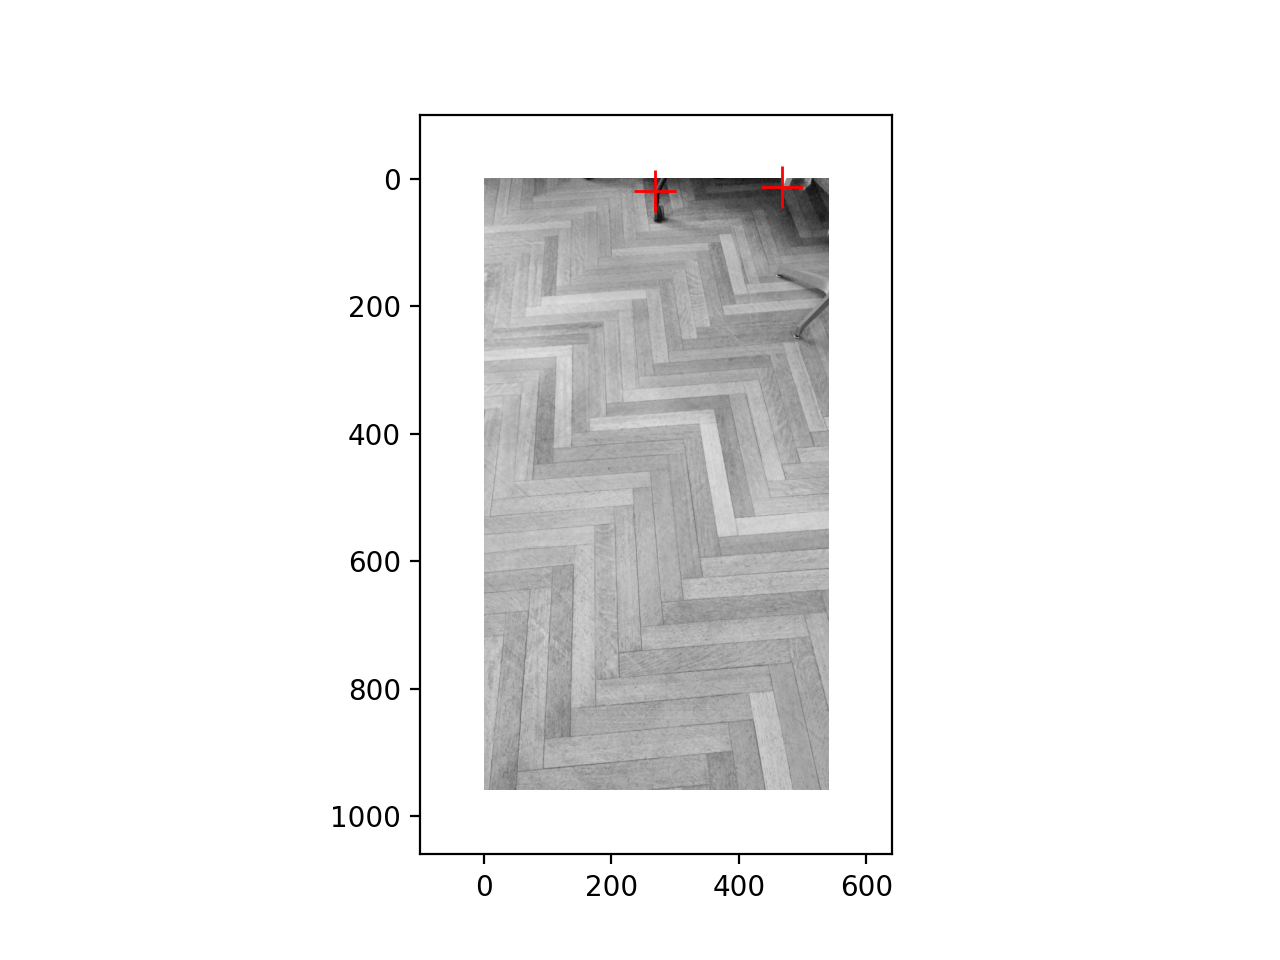
\includegraphics[width=0.49\linewidth]{Q1_RISHLibrary2.png}
    \caption{Left: RISHLibrary1.jpg; Right: RISHLibrary2.jpg}
\end{figure*}




\pagebreak
\paragraph{A1 (b):} Answer for Chase pair

The results are shown in Fig. 4. The corners returned for \texttt{Chase1.jpg} and \texttt{Chase2.jpg} are different. In left part, the corners returned are corners on sculpture while in right part, there is no corner returned though it is the same sculpture. This is because that the right image is not clear enough. Challenges in real life: sometimes the images we want to match might not be clear enough that the algorithm cannot detect any corners in the image. Let alone to match those images.

\begin{figure*}[htbp]
    \centering
    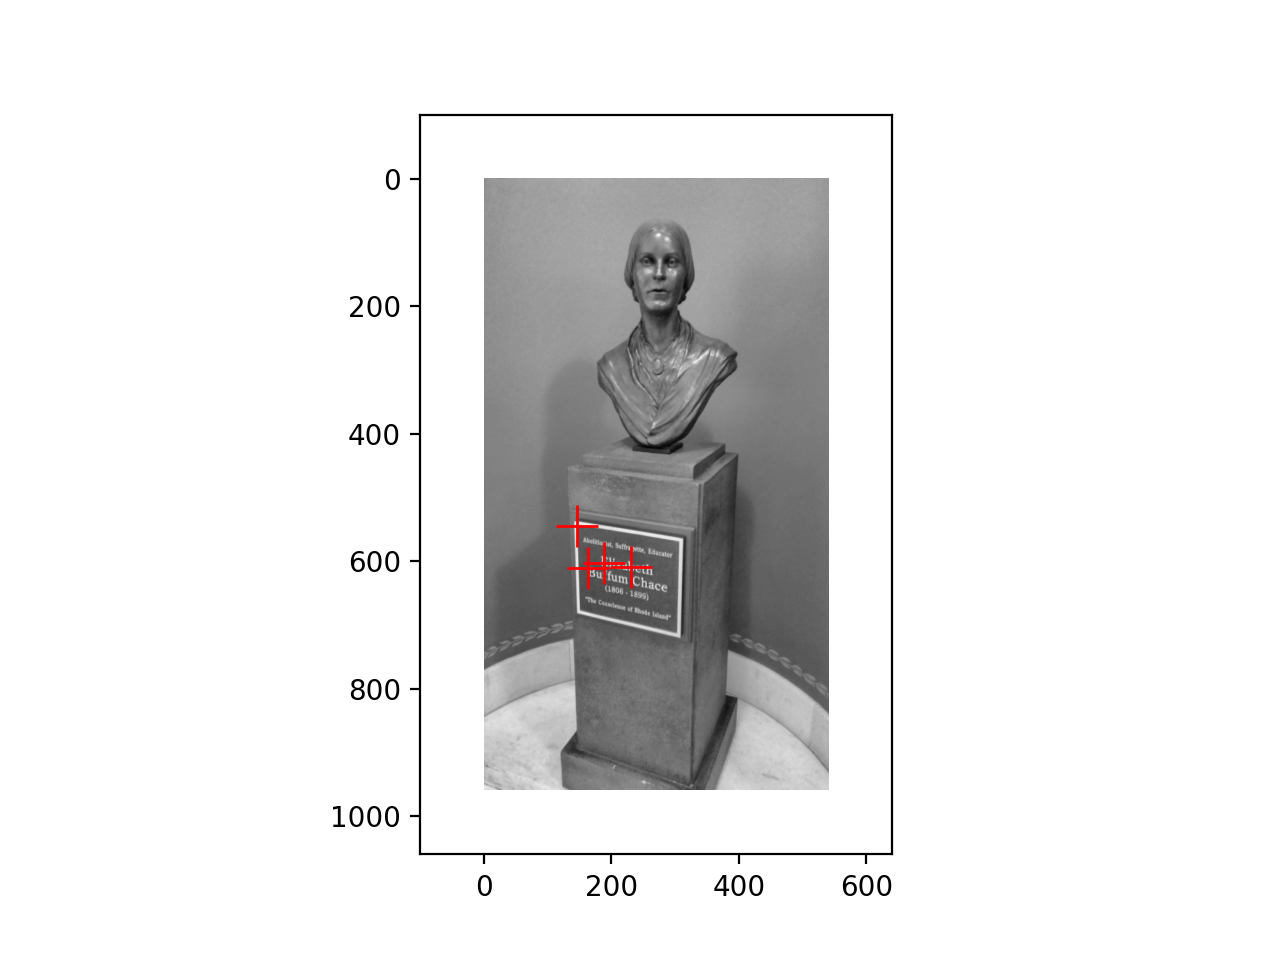
\includegraphics[width=0.49\linewidth]{Q1_Chase1.png}
    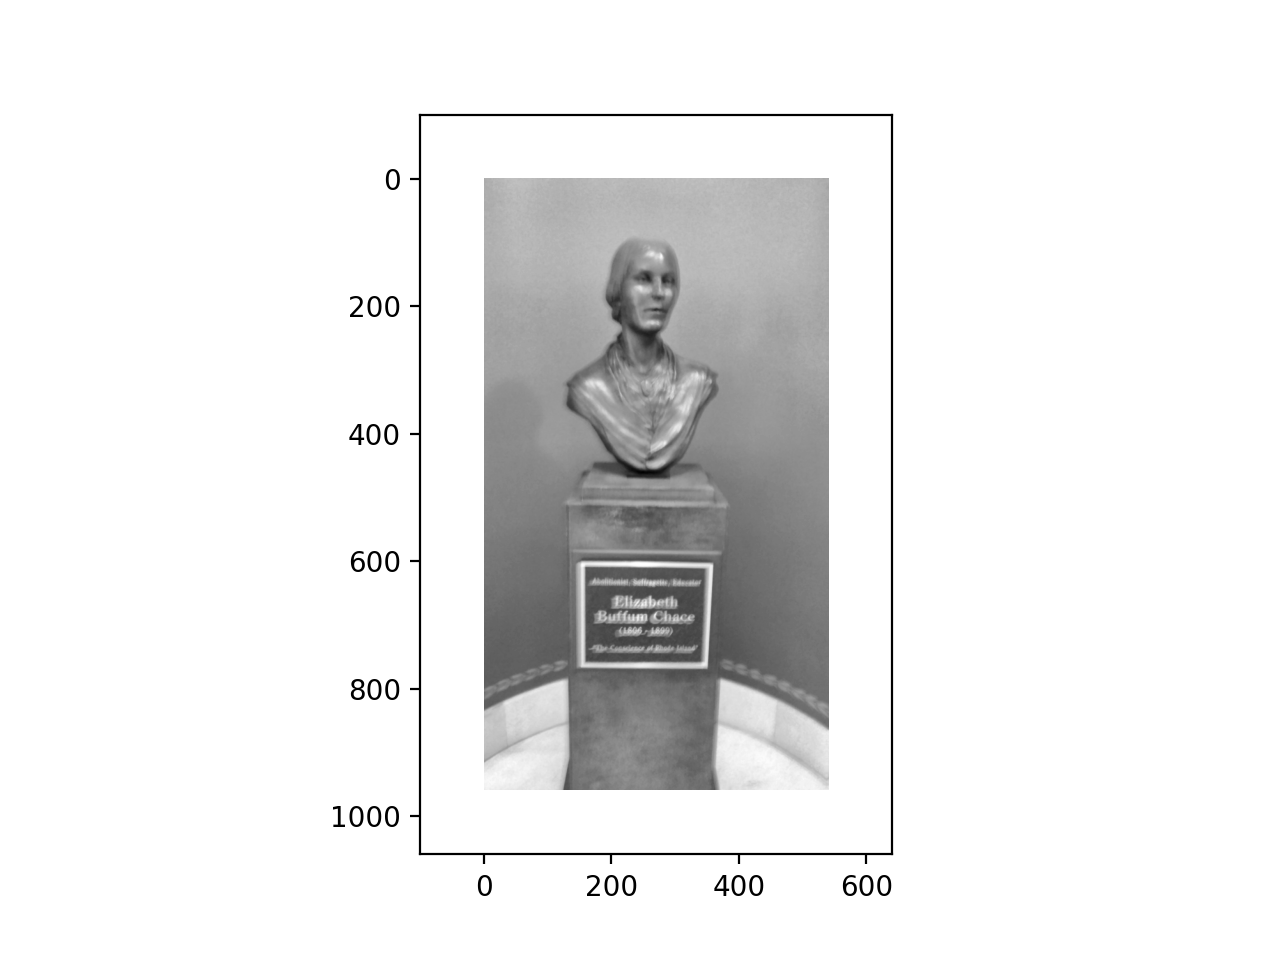
\includegraphics[width=0.49\linewidth]{Q1_Chase2.png}
    \caption{Left: Chase1.jpg; Right: Chase2.jpg}
\end{figure*}




\pagebreak
\paragraph{A1 (c):} Answer for LaddObservatory pair

The results are shown in Fig. 5. The corners returned for \texttt{Ch.jpg} and \texttt{Chase2.jpg} are different. There are more corners returned in right image because there are people in the image while they are not in the left image. In the meantime, for the static structure, most corners can match. Challenges in real life: the objects in the image can move which can result in the appearance or disapperance in the new image. The number of corners will increase or decrease correspondingly. And it might cause mismatch as last.

\begin{figure*}[htbp]
    \centering
    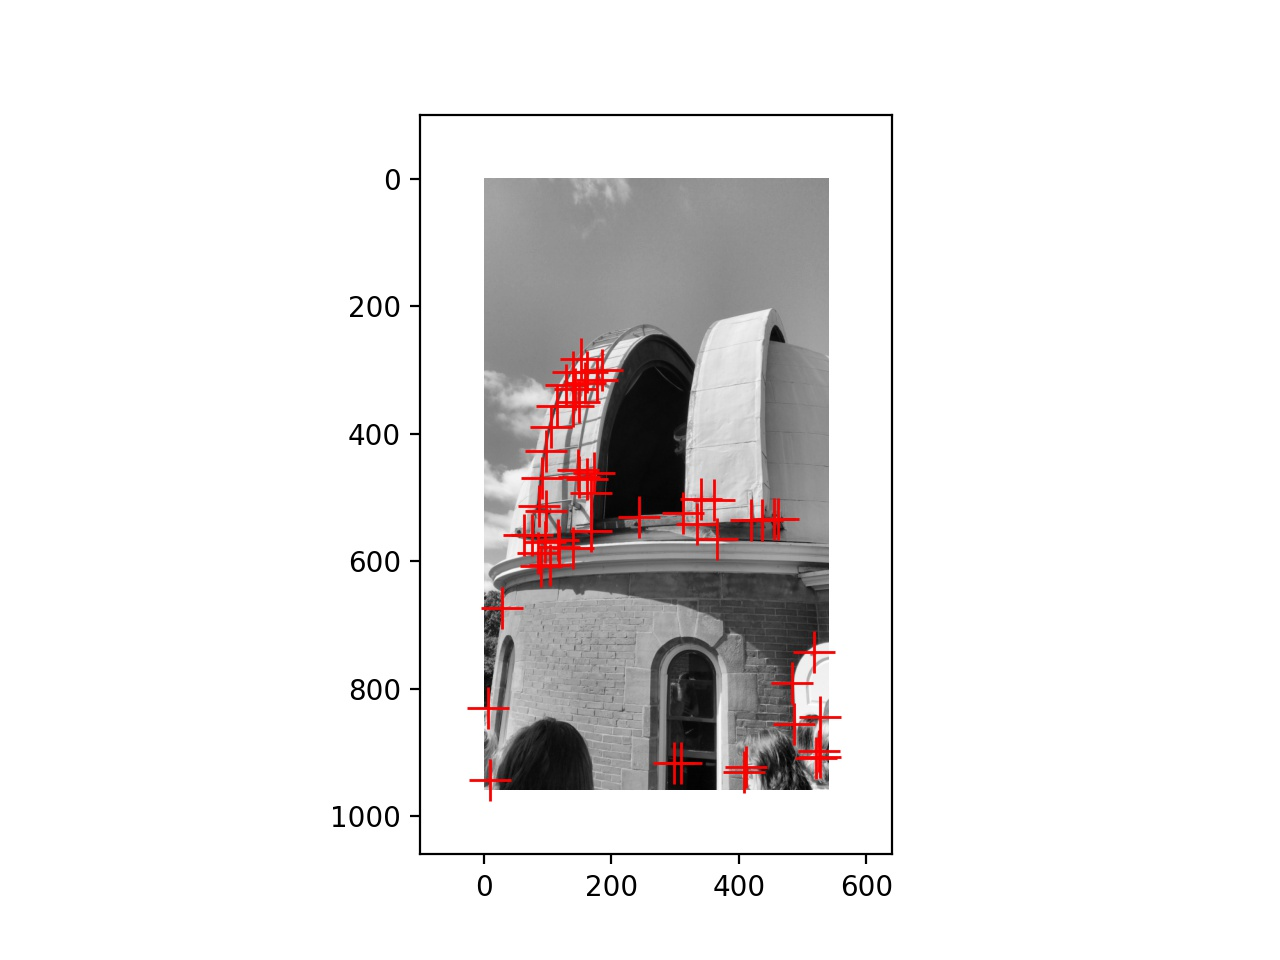
\includegraphics[width=0.49\linewidth]{Q1_LaddObservatory1.jpg}
    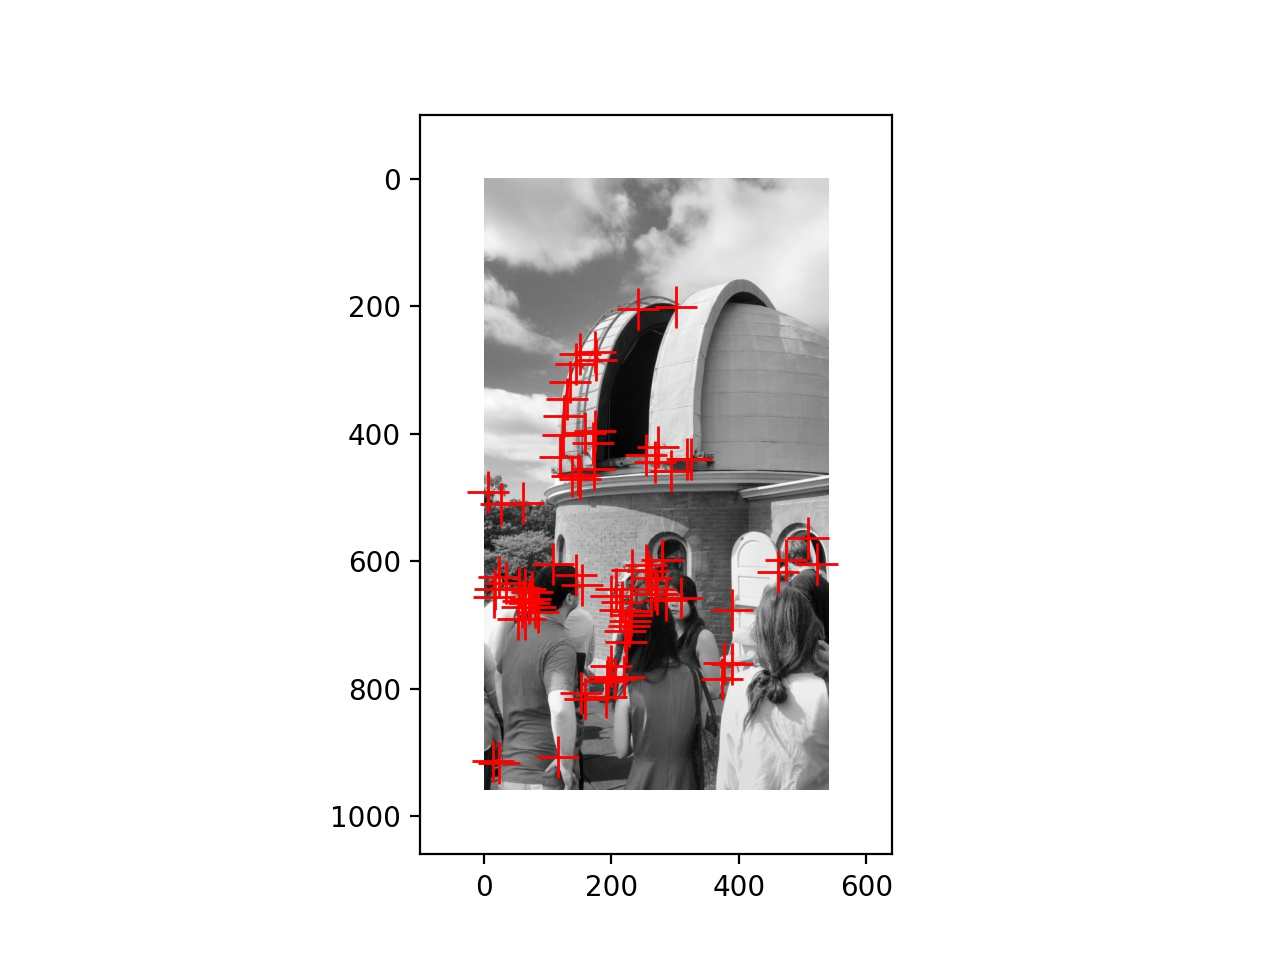
\includegraphics[width=0.49\linewidth]{Q1_LaddObservatory2.jpg}
    \caption{Left: LaddObservatory1.jpg; Right: LadObservatory2.jpg}
\end{figure*}




%%%%%%%%%%%%%%%%%%%%%%%%%%%%%%%%%%%

% Please leave the pagebreak

\pagebreak
\paragraph{Q2:}
The Harris Corner Detector is commonly used in computer vision algorithms to find locations from which to extract stable features for image matching.

How do the eigenvalues of the `M' second moment matrix vary with local image brightness, and how might we interpret the eigenvalues geometrically (think `shape')?

%%%%%%%%%%%%%%%%%%%%%%%%%%%%%%%%%%%
\paragraph{A2:} 
In Harris Corner Detector, $M$ is 
\begin{equation*}
    M = \sum\begin{bmatrix}
        I_x^2 & I_xI_y \\
        I_xI_y & I_y^2
    \end{bmatrix}
\end{equation*}
where $I$ is the gradient of corresponding direction, computed by the differences of the brightness of the pixels. And we use the $M$ to approximate the error function $E$ in following way,

\begin{equation*}
    E(u, v) \approx [u, v] M \begin{bmatrix}
        u \\ v
    \end{bmatrix}
\end{equation*}

By computing the gradient covariance matrix, we are fitting a quadratic to the gradients over a small image region. Thus, the surface $E(u, v)$ is locally approximated by a quadratic form. 

Interpret the eigenvalues geometrically: when $\lambda_2 \gg \lambda_1$, it implies a horizontal edge. When $\lambda_2 \sim \lambda_1$ and both are small values, it implies flat region. When $\lambda_2 \sim \lambda_1$ and both are big values, it implies a corner. When $\lambda_1 \gg \lambda_2$ and both are small values, it implies a vertical edge. The relations can be illustrated by the picture below.

\begin{figure*}[htbp]
    \centering
    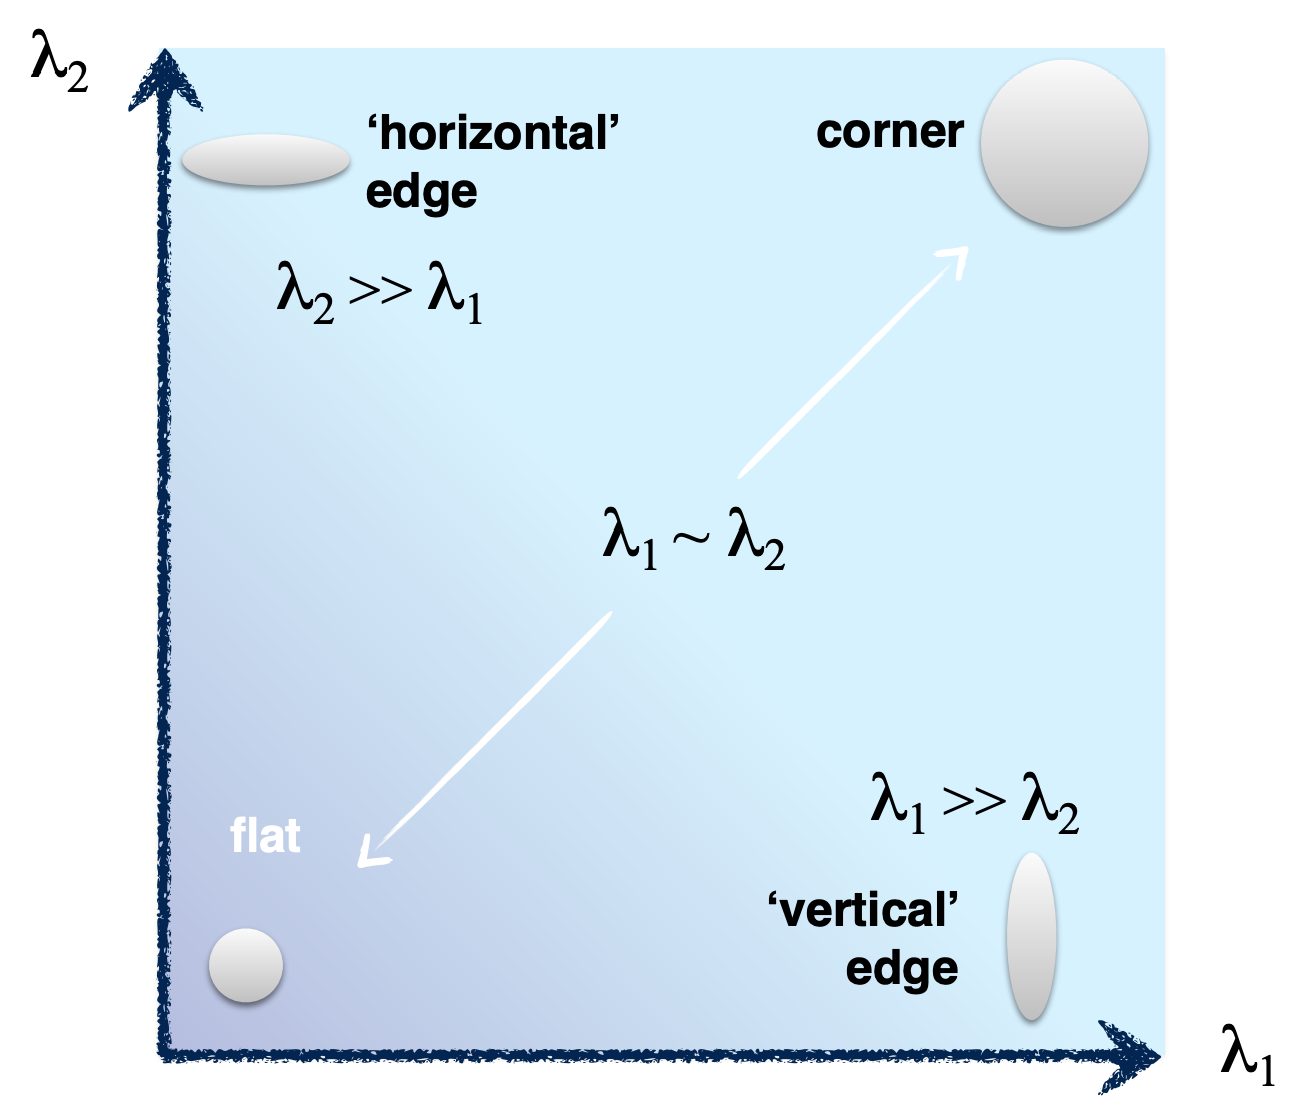
\includegraphics[width=0.5\linewidth]{eig_M_explaination.png}    
\end{figure*}

(source: http://www.cs.cmu.edu/\~16385/s17/Slides/6.2\_Harris\_Corner\_Detector.pdf)
%%%%%%%%%%%%%%%%%%%%%%%%%%%%%%%%%%%


% Please leave the pagebreak
\pagebreak
\paragraph{Q3:} Given a feature point location, the SIFT algorithm converts a 16$\times$16 patch around the feature point into a 128$\times$1 descriptor of the gradient magnitudes and orientations therein. Write pseudocode \emph{with matrix/array indices} for these steps.

\emph{Notes:} Do this for just one feature point at one scale; ignore the overall feature point orientation; ignore the Gaussian weighting; ignore all normalization post-processing; ignore image boundaries; ignore sub-pixel interpolation and just pick an arbitrary center within the 16$\times$16 for your descriptor. Please just explain in pseudocode how to go from the 16$\times$16 patch to the 128$\times$1 vector. You are free to simplify the gradient computation.

%%%%%%%%%%%%%%%%%%%%%%%%%%%%%%%%%%%
\paragraph{A3:} Your answer here.

\begin{python}
# You can assume access to the image, x and y gradients, and their magnitudes/orientations.

import numpy as np
from math import sqrt, atan2

image = imread('rara.jpg')
grad_x = filter(image, 'sobelX')
grad_y = filter(image, 'sobelY')
grad_mag = sqrt( grad_x .^2 + grad_y.^2 )
grad_ori = atan2( grad_y, grad_x )

# Takes in a feature point x,y location and returns a descriptor
def SIFTdescriptor(x, y):
    descriptor = np.zeros(128)

    bin_width = np.pi/4
    count = 0
    for col in range(0, image.shape[1], 4):
        for row in range(0, image.shape[0], 4):
            bins = np.zeros(8)
            for i in range(4):
                for j in range(4):
                    bins[int(grad_ori//bin_width)] += grad_mag
            descriptor[count:count+8] = bins
            count += 8

    return descriptor
\end{python}




%%%%%%%%%%%%%%%%%%%%%%%%%%%%%%%%%%%

% Please leave the pagebreak
\pagebreak
\paragraph{Q4:}
Digital cameras, computer networks, and computer storage have allowed us to build large sensor networks, and Brown is no exception in their use. The Brown Daily Herald has written about this practice \href{https://www.browndailyherald.com/2008/01/10/surveillance-cameras-on-campus-triple/}{both in 2008} and \href{https://www.browndailyherald.com/2020/02/21/cameras-installed-hegeman-hall/}{in 2020}---please read these articles in chronological order.

\emph{Please respond in 3-4 sentences to each question.}

\begin{enumerate}[(a)]
    \item What was your initial reaction to reading these articles twelve years apart?
    \item What arguments are made for the potential positives and negatives of having such a system at Brown?
\end{enumerate}

There are now about as many cameras at Brown as full-time faculty.

%
% NOT REQUIRED
% 
% With keen eyes, take a short walk to campus or to a local center and count the number of cameras that you see from start to finish. \\
% \emph{COVID-19: Please be responsible and respect social distancing and local norms; use good judgement and complete the exercise as best as you can. If you do not feel comfortable, it is of course appropriate to skip this question.}

% \begin{enumerate}[(c)]
%     \item Where are you, and how many cameras did you see? \\Were there any cameras inside your living space?
% \end{enumerate}

This much data is time consuming to process manually, but computer vision allows us to analyze captured image and video data automatically.
Since 2015, Brown’s primary supplier of surveillance cameras---Axis Communication---has \href{https://www.axis.com/customer-story/3767}{advertised} its cameras’ abilities to perform onboard facial recognition. But, the decision to use the function is left to the implementing organization.

\begin{enumerate}[(c)]
    \item Does knowing that this capability exists change your reaction? How?
\end{enumerate}

%%%%%%%%%%%%%%%%%%%%%%%%%%%%%%%%%%%
\paragraph{A4 (a):}
I am quite shocked when reading these two articles. I haven't noticed that there are many surveillance cameras among the campus before and cannot imagine that cameras are installed in common areas in residence halls. The trending of the installation of cameras is terrifying as it is taking our privacy step by step.

\paragraph{A4 (b):} \textbf{Pros:} 1. it can be utilized to assist in solving crime. 2. it can be used as a "patrol tool" and has a terrific deterrent value. \textbf{Cons:} 1. it can sacrifice the privacy of students. 2. it can cost a lot of money.



\paragraph{A4 (c):} It makes me feel more unconformtable about the cameras around the campus. The ability of analysis of the camera vedios implies that our data would be dealed in a third party company, which might result in data breach. I would prefer only processing the vedios within the university.


%%%%%%%%%%%%%%%%%%%%%%%%%%%%%%%%%%%
\newpage
Rather than fixed-in-place cameras, one way to reduce the number of cameras needed in outdoor environments could be to use mobile cameras attached to manually-operated drones. 

Drones are often used by individuals, companies, and governments for photography, with some organizations demonstrating delivery applications, too. In the U.S., the federal government has started using drones for domestic surveillance---please read the \href{https://www.eff.org/issues/surveillance-drones}{Electronic Frontier Foundation}'s summary. Drone surveillance may improve security, but it may also degrade personal privacy.

% ``Drones already in use by law enforcement can carry various types of equipment including live-feed video cameras, infrared cameras, heat sensors, and radar. Some military versions can stay in the air for hours or days at a time, and their high-tech cameras can scan entire cities, or alternatively, zoom in and read a milk carton from 60,000 feet. They can also carry WiFi crackers and fake cell phone towers that can determine your location or intercept your texts and phone calls. Drone manufacturers even admit they are made to carry “less lethal” weapons such as tasers or rubber bullets."

% Drone surveillance may improve security, but it may also degrade personal privacy. \\
Imagine that Brown's Department of Public Safety purchased a drone fleet, and built its recharging station atop the Science Library. 

\begin{enumerate}[(d)]
    \item Under what conditions would you be comfortable with security drones around campus?
\end{enumerate}

%%%%%%%%%%%%%%%%%%%%%%%%%%%%%%%%%%%
\paragraph{A4 (d):} The only condition that I can think about being comfortable with security drones around is when the campus is unsafe for people to stay, for example, walking alone at midnight. We have heard many crime cases happened around the campus last year at night. It will make people feel safer if they could see drones flying on their way back home.




%%%%%%%%%%%%%%%%%%%%%%%%%%%%%%%%%%%
\newpage
Drones could become automatic to operate, and  \href{https://link.springer.com/article/10.1007/s10846-017-0483-z}{drones use increasingly-sophisticated computer vision} to aid control. In Project 2, we learn about feature detection, description, and matching algorithms to provide correspondence between images. When applied to video, this allows drones to estimate their motion relative to the world. Please \href{https://www.youtube.com/watch?v=jIvJuWdmemE}{watch this video} for a demonstration---at one minute in, we see the real-time feature matching in the bottom left.

As such, cameras and image correspondence are foundational technologies for reliable drone localization and navigation. This enables assisted or even autonomous flying in complex environments, such as for \href{https://www.cnn.com/2019/05/01/health/drone-organ-transplant-bn-trnd/index.html}{life-saving organ delivery}. Yet, adding cameras to drones also makes them potentially capable as autonomous surveillance platforms.

\begin{enumerate}[(e)]
    \item With respect to cameras, what solutions might we consider to reconcile a desire for useful drones with a desire for privacy? \\
    \emph{These might be technological, sociological, legal, etc.---wide scope.}
\end{enumerate}

%%%%%%%%%%%%%%%%%%%%%%%%%%%%%%%%%%%
\paragraph{A4 (e):} There can be many ways to reconcile the desire for useful drones with a desire for privacy. For example, techiniquelly, when the drone is flying and using the images captured by cameras for navigation, we could apply a mask to the faces of people that the cameras have captured so that the drone won't be able to detect face. And considering the storage of the videos, it would be possible to make some rules or laws regulating how the manufacturers of drones should store those information. Moerover, we could also set specific areas for drones and in those areas we could set up signs telling people about the potential of appearing in cameras.






%%%%%%%%%%%%%%%%%%%%%%%%%%%%%%%%%%%


%
% NOT REQUIRED
%

% % Please leave the pagebreak
% \pagebreak
% \paragraph{Q5:} Distance metrics for feature matching.

% \begin{enumerate}[(a)]
%     \item Explain the differences between the geometric interpretations of the Euclidean distance and the cosine similarity metrics. What does this tell us about when each should be used?
% \end{enumerate}

% %%%%%%%%%%%%%%%%%%%%%%%%%%%%%%%%%%%
% \paragraph{A5 (a):} Your answer here.




% %%%%%%%%%%%%%%%%%%%%%%%%%%%%%%%%%%%

% \pagebreak
% \begin{enumerate}[resume*]
%     \item Given a distance metric, what is a good method for feature descriptor matching and why?
% \end{enumerate}

% %%%%%%%%%%%%%%%%%%%%%%%%%%%%%%%%%%%
% \paragraph{A5 (b):} Your answer here.




%%%%%%%%%%%%%%%%%%%%%%%%%%%%%%%%%%%

%
% NOT REQUIRED
%

% \pagebreak
% \paragraph{Secret `something to think about' (ungraded):} 
% In designing a feature point matching algorithm, what characteristics might we wish it to have? How might two world points change in appearance across photographs? Consider that we might allow brightness or contrast changes, or texture changes, or lighting changes, or geometric changes in appearance like rotation and translation in three dimensions or camera perspective effects. All exist between some two photographs of real-world points. 

% We are faced with a fundamental trade-off between feature point invariance (how much variation in appearance I allow and still say that two points are the same) and discriminative power (our ability to say that two points are different or the same at all). 

% How should we design for this trade-off?


\pagebreak
\section*{Feedback? (Optional)}
Please help us make the course better. If you have any feedback for this assignment, we'd love to hear it!


% \pagebreak
% \section*{Any additional pages would go here.}



\end{document}
